\begin{figure}[t]
\centering
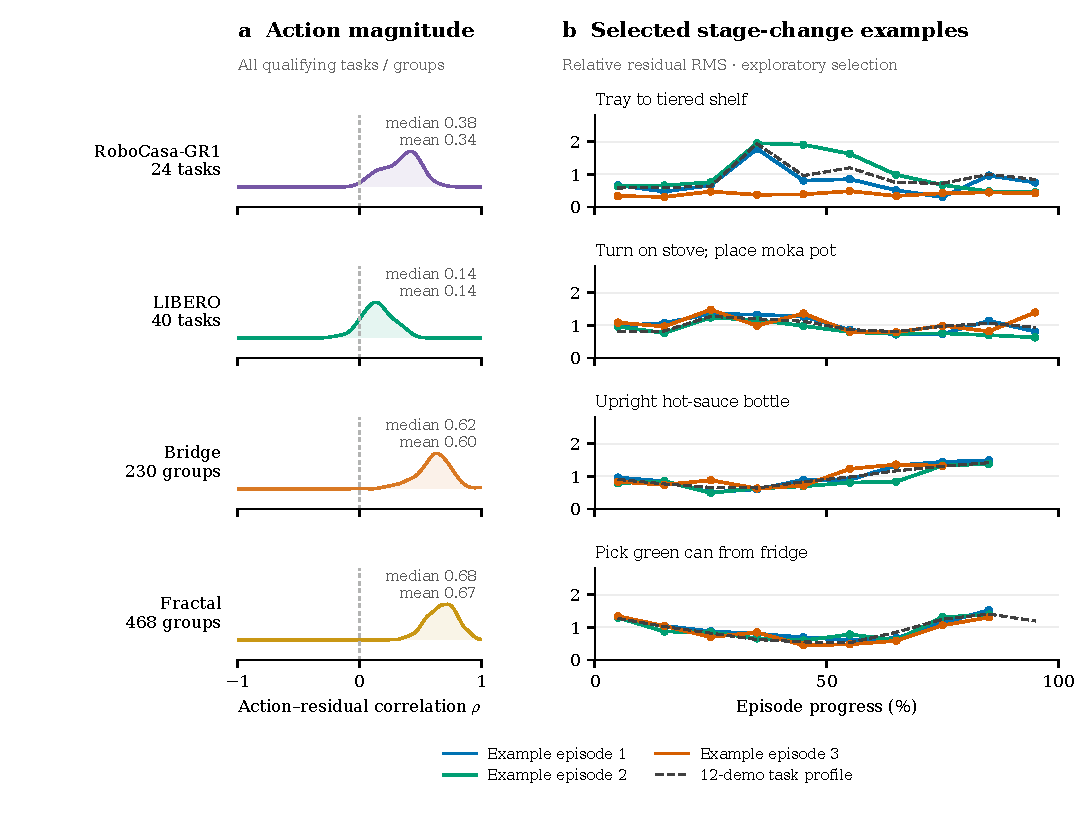
\includegraphics[width=\linewidth]{analysis/diagnostics/crossdataset_residual/all_datasets_progress_selected_trajectories.pdf}
\caption{\textbf{Action magnitude and examples of stage-dependent regression residuals.}
(a) Task-wise action--residual correlations across all qualifying tasks or instruction
groups; the empirical values are unchanged from the full-coverage analysis.
(b) Three selected demonstration episodes from one task per dataset, with the
12-demonstration task profile dashed. Tasks are selected for a large stage-scale
contrast recurring across two episode halves; the three episode shapes closest to
the task profile are displayed. This is exploratory, effect-based selection for
illustration, not an estimate of prevalence or an independent validation test.
Each curve uses a common task-level normalization and the existing ten progress-bin
samples, without smoothing or temporal alignment. Binary grippers are excluded;
GR1 hand joints are retained. All residuals come from general-MSE policies evaluated
on training demonstrations.}
\label{fig:selected-progress-examples}
\end{figure}
